\section{Architecture}

% writing the architecture of the model
A DeepLabv3 model with Resnet-101 backbone and FCN auxilary classifier is trained with data. 

\subsection{DeepLabv3}

DeepLabv3 is a semantic segmentation model that uses Atrous convolution to capture multi-scale context by using different dilation rates. It uses a ResNet-101 backbone with atrous convolution. The model uses atrous spatial pyramid pooling (ASPP) to capture multi-scale context by using different dilation rates. The model also uses a fully connected conditional random field (CRF) to refine the segmentation results. 
It take N feature maps as input from the ResNet-101 backbone and outputs N*4*H*W tensor, where N is the batch size, 4 is the number of classes, H is the height, and W is the width of the image.The model outputs a probability distribution over the classes for each pixel in the input image.  
\begin{figure}[ht]
    \centering
    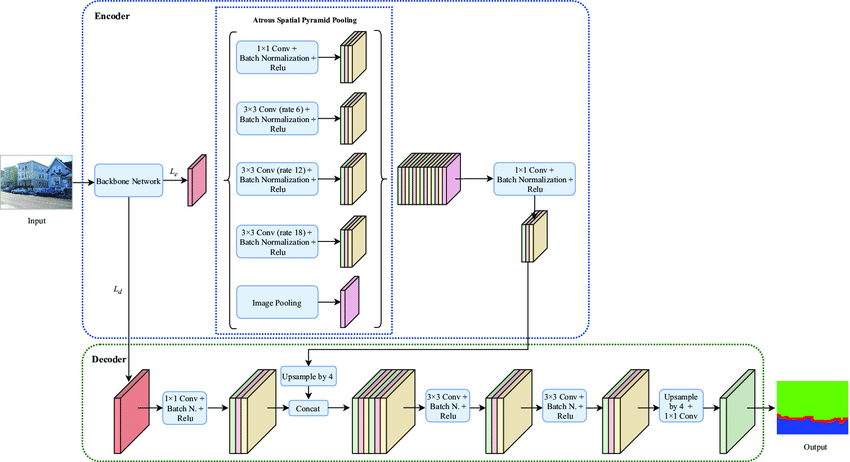
\includegraphics[width=0.6\textwidth]{Images/deeplabv3.png}
    \caption{DeepLabv3 architecture~\cite{deeplabv3-image}}
    \label{fig:deeplabv3}
\end{figure}

\begin{figure}[ht]
    \centering
    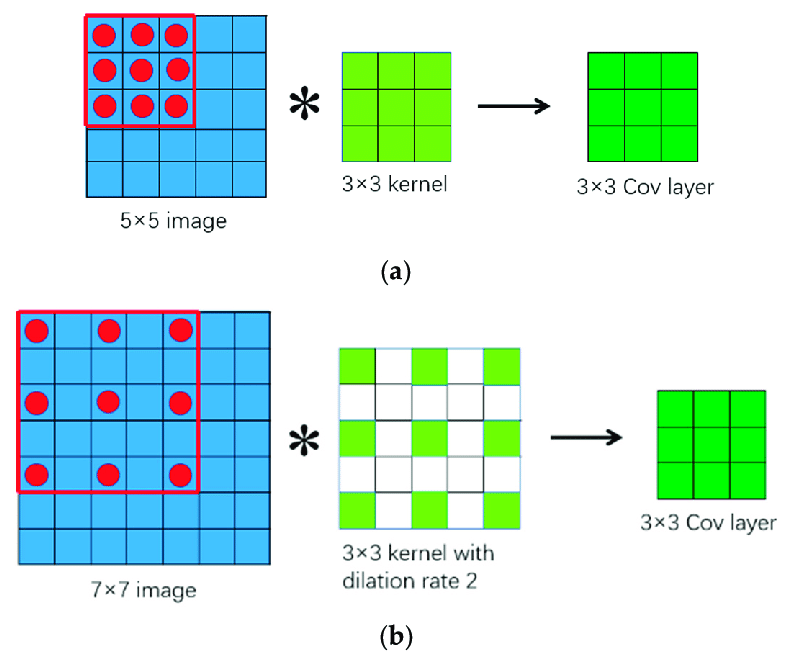
\includegraphics[width=0.5\textwidth]{Images/atrous-convolution.png}
    \caption{Atrous Spatial Pyramid Pooling (ASPP) in DeepLabv3\\ (a) Conv 3x3, rate=1 (b) Conv 3x3, rate=2 \\
    \cite{atrous-convolution-image}}
    \label{fig:atrous-convolution}
\end{figure}


\subsection{MobileNetV3-Large Backbone}

MobileNetV3-Large is a convolutional neural network designed for feature extraction. MobileNetV3-Large architecture uses 16 initial filters in the first convolution layer and then reduces the number of filters in the later layers by a factor of 2. It has typically 60 layers. Its building block involves an Inverted Residual Block, which includes a depth-wise convolution, a squeeze-and-excitation module, and a point-wise convolution. It takes normalized RGB im-
ages as input and outputs feature maps that are used by the
DeepLabv3 and the auxilary classifier. Input to the layer is
a 4-dimensional tensor with normalized RGB channels, and
the output is N*32*32, where N is the batch size. It involves downsampling layers.

\begin{figure}[ht]
    \centering
    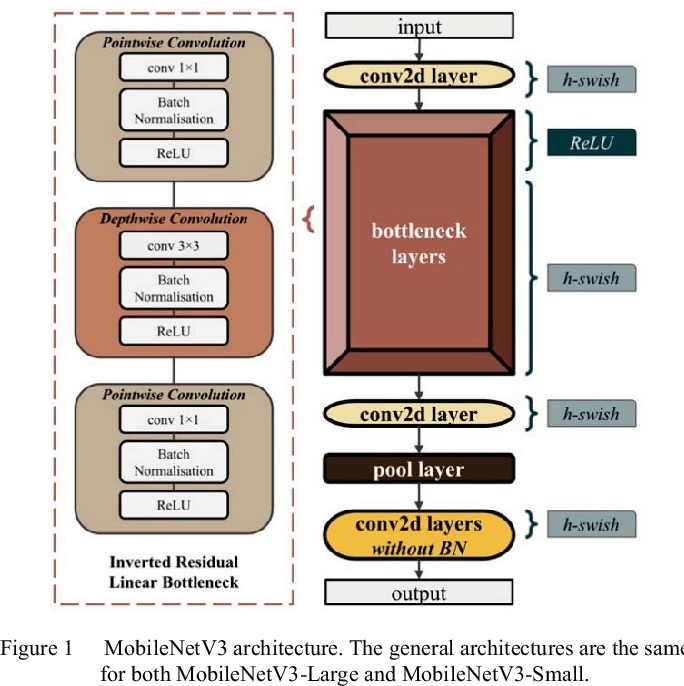
\includegraphics[width=0.5\textwidth]{Images/mobilenet-1.png}
    \caption{\cite{mobilenet-1}}
    \label{fig:mobilenet-1}
\end{figure}

\begin{figure}[ht]
    \centering
    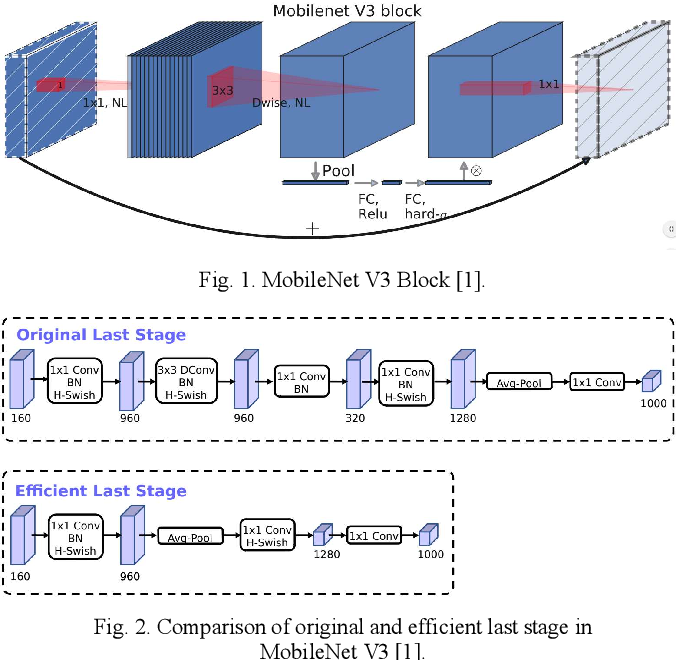
\includegraphics[width=0.5\textwidth]{Images/mobilenet-2.png}
    \caption{\cite{mobilenet-2}}
    \label{fig:mobilenet-2}
\end{figure}

\subsection{Training Setup}
While training on data, the input is a 4-dimensional tensor with normalized RGB channels, and the labels are 2D tensors with integer values representing the class labels for each pixel. The output from the PyTorch model is a 4-dimensional tensor with the shape (N, 4, H, W), where N is the batch size, 4 is the number of classes, H is the height, and W is the width of the output. The output is a probability distribution over the classes for each pixel in the input image. \\
The model is trained with the cross-entropy loss function, which is minimized using the Adam optimizer. The model is trained for 40 epochs. The learning rate is set to 0.01. The training takes approximately 30 mins to complete. The model is evaluated 3 images. The evaluation metrics used are precision, mean intersection over union (mIoU) and pixel accuracy.
